\clearpage
\section{Hardware}\label{sec:Hardware}
Das \textit{Machine Controlling System} dient der Steuerung des 3D-Druckers sowie der Regelung einzelner Komponenten. Es setzt sich aus mehreren funktional verschiedenen Einheiten zusammen, welche in diesem Kapitel beschrieben werden.


\subsection{Bluetooth Mesh Node}\label{subsec:BMN}
Im Bluetooth Mesh Protokoll gibt es zwei verschiedene arten Geräte, in "unprovisioned device" und einen "Node". Das "unprovisioned device" ist ein Teilnehmer, der unbekannt für das Mesh Netzwerk ist und deshalb keine Rechte besitzt. Wird dieses Gerät nun in das Netzwerk aufgenommen, so wird das "unprovisioned device" zu einem Node. Dieses vorgehen nennt sich "provisioning". Die Hardware für den Node besteht bei allen Geräten aus dem gleichen SoC. Der NRF52840 von Nordic Semiconductor eignet sich aus folgenden Gründen perfekt für diese Anwendung. Die Nodes dürfen um eine lange Laufzeit zu generieren, sehr wenig elektrische Leistung beziehen. Der NRF52840 benötigt im Ruhemodus nur wenige micro Ampere. Ein weiterer Grund ist die sehr gute Dokumentation der Software von Nordic Semiconductor. Die gesamte Software ist im Infozenter erhältlich und frei zugänglich. Weitere Forteile befinden sich in der nachfolgenden Tabelle:

\begin{figure}[h]
	\centering
	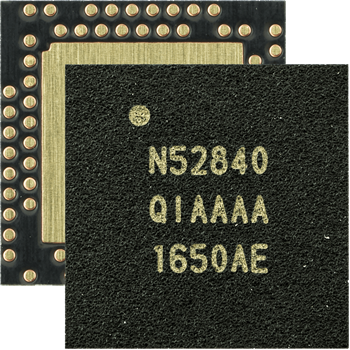
\includegraphics[scale=0.5,angle=0]{nRF52840.png}
	\caption{nRF52840 SoC}
	\label{img:nRF52840}
\end{figure} 

\subsection{Debugging Interface Unit (DIU)}\label{subsec:DIU}
Die \textit{Debugging Interface Unit} ist dazu da, das Debuggen während dem Entwicklungsprozess der Firmware zu vereinfachen. Via UART/USB-Bridge können Messwerte, Statewerte der aktuell verwendeten Zustandsmaschinen, etc. auf dem Computer ausgegeben werden. Aus Kostengründen würden die verwendeten Bauteile in einer Serienproduktion nicht bestückt werden und stellen daher eine Bestückungsvariante dar.

\subsection{Printer Controlling Unit (PCU)}\label{subsec:PCU}
Die \textit{Printer Controlling Unit} beinhaltet die nötige Schaltungsteile um den 3D-Drucker zu steuern bzw. zu regeln. Namentlich den zentralen Mikrocontroller und diverse Bussysteme welche nötig sind um die verwendete Peripherie anzusteuern. Als Grundlage für die Firmware des Mikrocontrollers wird die Firmware \textit{Marlin} verwendet \cite{marlin_webseite} welche unter \textit{GNU General Public License Version 3} frei verfügbar ist \cite{marlin_gnu_lizenz}. Aus Kompatibilitätsgründen zu den erforderlichen Pins der Firmware \textit{Marlin} wird als Mikrocontroller ein \textit{ATmega2560} \cite{ATmega2560_spezifiaktion} der Firma \textit{Microchip Technology} verwendet.

\subsection{Storage Disk Unit (SDU)}\label{subsec:SDU}
Die \textit{Storage Disk Unit} besteht aus einem SD-Karten-Slot sowie aus dessen Ansteuerung. Diese dient dazu G-Code Dateien (zu druckende 3D-Modelle), welche via WLAN empfangen werden, zwischenzuspeichern oder kann direkt als Quelle für G-Code Dateien dienen. Die SD-Karte ist via SPI (\textit{Serial Peripheral Interface}) an den Mikrocontroller angeschlossen. 

\subsection{Heater-Fan-Controll Unit (HFU)}\label{subsec:HFU}
Die \textit{Heater-Fan-Controll Unit} dient dazu die Ventilatoren sowie die Heizelemente in Heizbett und Extruder anzusteuern und zu regeln. Dazu wird ein Regelungssystem bestehend aus Ventilator bzw. Heizung und Temperatursensor aufgebaut, welches von der \textit{Printer Controlling Unit} gesteuert wird. Alle Aktoren können per Pulsweitenmodulation (PWM) oder per Ein/Aus Steuerung geregelt werden. Beim Heizbett muss darauf geachtet werden das die spezifizierte Maximaltemperatur von $110^\circ$C \cite{ender3_spezifiaktion} nicht überschritten wird.

\subsection{Interface Controlling Unit (ICU)}\label{subsec:ICU}
Die \textit{Interface Controlling Unit} dient dazu via WLAN eine Verbindung zum Internet herzustellen und somit G-Code Dateien (zu druckende 3D-Modelle) zu empfangen und diese an die \textit{Printer Controlling Unit} weiterzuleiten. Ausserdem können Befehle empfangen werden welche z.B. die Schrittmotoren steuern. Um den Verbindungsaufbau zu vereinfachen wird auf ein vorgefertigtes \textit{ESP8266} Modul zurückgegriffen \cite{ESP8266_spezifiaktion}.


\subsection{Human-Machine-Interface (HMI)}\label{subsec:HMI}
Das \textit{Human-Machine-Interface} bietet dem Benutzer neben dem \textit{Human-Machine-System} eine sekundäre Option, um mit dem 3D-Drucker zu interagieren. Es setzt sich aus einem Drehgeber und einem Display (voraussichtlich \textit{LCD12864} der Firma \textit{Waveshare}) zusammen. Auf letzterem werden verschiedene Optionen und Statusanzeigen dargestellt, auf welche durch Verwendung des Drehgebers zugegriffen werden kann.


\subsection{Power Management Unit (PMU)}\label{subsec:PMU}
Als Speisung für die gesamte Hardware ist das mitgelieferte Netzteil des \textit{Ender 3} 3D-Druckers ($24 VDC$ / $15A$) vorgesehen. 
%Da dieses möglicherweise nicht genügend Strom zur Verfügung stellt, ist angedacht es bei Bedarf während des Entwicklungsprozesses mit einem ATX-Netzteil\footnote{\textbf{ATX} steht für \textit{Advanced Technology Extended}. Diese Netzteile werden normalerweise in Desktop Computer verbaut und liefern $12VDC$, $5VDC$ und $3.3VDC$ und sind mit Leitungen von $100W$ bis zu $2000W$ verfügbar.} zu ersetzen.

Um die genaue Leistungsaufnahme des Gerätes besser bestimmen zu können soll hier eine kurze Überschlagsrechnung gemacht werden. Die Bauteile, die die grösste Auswirkung auf die Leistungsaufnahme haben sind: 4 x Steppermotor, Heizbett und die Extruder Heizung. Die anderen Komponenten können im Vergleich vernachlässigt werden. Ein einziger Motor hat einen maximalen Strom von 2.5A, eine Betriebsspannung von 3.1V und somit eine maximale Leistung von 7.7W \cite{steppermotor}. Das Heizbett wird mit 24V gespiesen und hat eine Leistung von 220W \cite{Heizbett_Ender3}.
%Das Heizbett wird mit $24V$ gespiesen, hat einen gemessenen Widerstand von ??$\Omega$ und damit eine Leistung von ??$W$. 
Die Extruder Heizung hat nach Hersteller eine Leistung von 40W \cite{Extruder_Heizung}. Somit ergibt sich, mit eine maximale Leistung von $\sim290$W für diese wichtigen Bauteile.

Das von \textit{Creality3D} bereitgestellte Netzteil mit $\sim360$W ist somit für unsere Zwecke gut dimensioniert und muss nicht geändert werden \cite{ender3_spezifiaktion}. 

%Die Motoren arbeiten jedoch effektiv nie bei diesen Strömen. Höhere Ströme sind nur möglich, wenn die Motoren viel Kraft benötigen. Dies ist jedoch in der vorliegenden Anwendung nicht der Fall, da das System so leichtgängig wie möglich sein sollte. Der verwendete Treiber gemäss Kapitel \ref{subsec:MCU} ist deshalb auch nicht für den Maximalstrom von $2.5A$ dimensioniert. Dazu kommt auch noch, dass die Motoren erst anfangen zu arbeiten, wenn die Heizelemente die Temperatur erreicht haben und somit nur noch die Temperatur halten müssen. Dies benötigt weniger Leistung als das Aufheizen selbst. Somit ist das Netzteil für unsere Zwecke wiederum überdimensioniert.










